\documentclass{article}
\usepackage{graphicx} % Required for inserting images
\usepackage[left=4cm, right=4cm, top=4cm, bottom=4cm]{geometry}
\usepackage[T1]{fontenc}
\usepackage[polish]{babel}
\usepackage{amssymb}
\usepackage{url}
\usepackage{enumitem}
\usepackage{dirtree}
\usepackage[export]{adjustbox}
\usepackage{amsmath}



\title{\Huge JIMP2 Projekt 2025 \\ {\huge Dokumentacja końcowa - C}}
\author{Michał Ludwiczak \\ GR3}
\date{29 kwietnia 2025}

\begin{document}

\maketitle

\tableofcontents



\section{Cel projektu}

Celem projektu jest stworzenie aplikacji w języku C, dokonującej podziału grafu na określoną przez użytkownika lub domyślną liczbę 2 równych części z zachowaniem wybranego lub, ponownie, domyślnego 10-procentowego marginesu różnicy. Liczba wierzchołków w powstałych częściach grafu nie powinna się różnić o więcej niż zadany margines procentowy, a liczba przeciętych krawędzi pomiędzy wynikowymi częściami grafu powinna być jak najmniejsza. Wyjściem programu ma być plik tekstowy lub binarny. Użytkownik ma mieć możliwość wskazać wyjście programu, a więc plik tekstowy lub binarny, zawierający wynik działania programu, oraz dane wejściowe, które mogą być wykorzystane ponownie w kolejnym działaniu programu.



% wizualizacja problemu
\begin{figure}[ht]
    \centering
    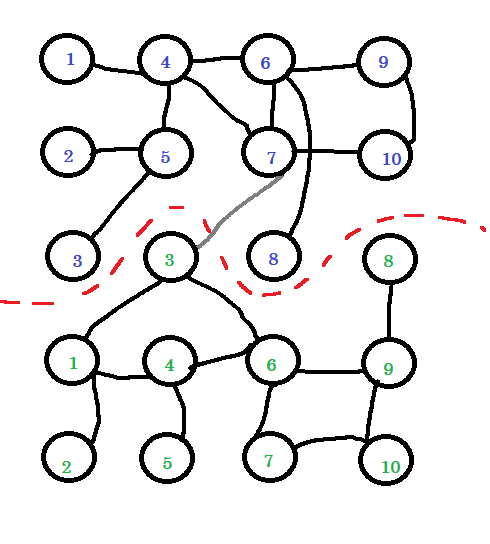
\includegraphics[width=0.75\linewidth]{img/graph.png}
    \caption{Przykładowy graf podzielony na 2 równe części}
    \label{fig:graph}
\end{figure}



\section{Algorytm}

Niestety znalezienie optymalnego podziału grafu należy do klasy problemów NP-trudnych. Dla grafu o \( n \) wierzchołkach istnieje aż \( 2^{n-1} - 1 \) możliwych sposobów na bisekcję (wyraźnego podziału na 2 grafy). \cite{youtube_video} Przy tego typu problemie nie możemy po prostu sprawdzić wszystkich możliwości i wybrać najlepszej z nich - jest to problem optymalizacji kombinatorycznej. W związku z tym opracowano wiele algorytmów zachłannych, metod przybliżonych i heurystyk, które pozwalają na uzyskanie satysfakcjonujących rozwiązań w praktyce.
W tym programie zdecydowałem się użyć algorytmu spektralnego, który wykorzystuje własności spektralne macierzy Laplace'a grafu. Na podstawie spektrum grafu, które opisuje strukturę jego strukturę, graf możemy podzielić w efektywny i satysfakcjonujący sposób, minimalizując liczbę przeciętych krawędzi.



    \subsection{Macierz Laplace'a}
    
    W podejściu spektralnym do podziału grafu kluczową rolę odgrywa macierz Laplace'a \cite{laplacian_matrix}.
    Wzór na Laplacian klasyczny definiuje się jako:
    \[
    \mathbf{L} = \mathbf{D} - \mathbf{A}
    \]
    gdzie:
    \begin{itemize}
      \item \( L \) to \textbf{macierz Laplace'a} grafu,
      \item \( D \) to \textbf{macierz stopni} to macierz diagonalna, w której elementy na diagonali \( d_{ii} \) odpowiadają stopniowi wierzchołka \( i \), czyli liczbie krawędzi, które są z nim bezpośrednio połączone. W przypadku pętli, każda taka krawędź zwiększa stopień wierzchołka o 2, ponieważ jest traktowana jako dwie krawędzie incydentne z tym samym wierzchołkiem
      \item \( A \) to \textbf{macierz sąsiedztwa} grafu, gdzie elementy \( a_{ij} \) są równe 1, jeśli istnieje krawędź między wierzchołkami \( i \) i \( j \), oraz 0 w przeciwnym przypadku.
    \end{itemize}
    


    \subsection{Metoda Lanczosa}

    Następnym krokiem jest obliczenie \(k = p - 1\) (gdzie p to liczba części, na które graf ma być podzielony) najmniejszych wektorów własnych, nie wliczając pierwszego zerowego. Dla bisekcji będzie to tylko jeden wektor, drugi najmniejszy - wektor Fiedlera. Wektory własne macierzy Laplace'a grafu przechowują informacje o połączeniach pomiędzy wierzchołkami. 
    Istnieje metoda Lanczosa \cite{lanczos}, którą można zastosować na macierzy Laplace'a, gdyż jest to macierz symetryczna, a więc również i hermitowska. Generuje ona ortonormalną bazę przestrzeni Kryłowa oraz przekształca macierz Laplace'a do macierzy trójdiagonalnej \(T\). Z wartości i wektorów własnych tej uproszczonej macierzy i bazy Kryłowa można obliczyć przybliżenia wartości i wektorów własnych oryginalnej macierzy. Dodatkowo wybór odpowiedniego wektora początkowego jest istotny dla efektywności metody. Często wybiera się go losowo, aby zapewnić, że ma składowe we wszystkich kierunkach przestrzeni własnej macierzy. Metoda Lanczosa może być również jednak podatna na niestabilności numeryczne, zwłaszcza w przypadku dużych macierzy. Aby temu przeciwdziałać, często stosuje się techniki ponownej ortogonalizacji. 


    \subsection{Algorytm QR}
    W celu obliczenia wartości własnych macierzy trójdiagonalnej \( \mathbf{T} \), uzyskanej z metody Lanczosa, zastosowano algorytm QR z rotacjami Givensa. Macierz \( \mathbf{T} \) jest rzeczywista, symetryczna i trójdiagonalna, co umożliwia efektywne wykorzystanie tego algorytmu.
    Algorytm polega na iteracyjnym rozkładzie macierzy \( \mathbf{T} \) na iloczyn macierzy ortogonalnej \( \mathbf{Q} \) i macierzy górnotrójkątnej \( \mathbf{R} \), a następnie aktualizacji \( \mathbf{T} \) poprzez mnożenie \( \mathbf{R} \mathbf{Q} \). Rotacje Givensa są stosowane do wyzerowania elementów poddiagonalnych, co zachowuje trójdiagonalność macierzy i redukuje złożoność obliczeniową.
    W każdej iteracji aktualizowana jest macierz \( \mathbf{Q}_{\text{total}} \), która akumuluje iloczyn wszystkich rotacji Givensa, umożliwiając późniejsze obliczenie wektorów własnych. Proces powtarza się, aż do osiągnięcia zbieżności, czyli gdy elementy poddiagonalne macierzy \( \mathbf{T} \) stają się wystarczająco małe. Po zbieżności, wartości własne odczytywane są z diagonali macierzy \( \mathbf{T} \), a wektory własne są kolumnami macierzy \( \mathbf{Q}_{\text{total}} \).
    Algorytm QR z rotacjami Givensa jest szczególnie efektywny dla macierzy trójdiagonalnych, ponieważ każda rotacja wpływa tylko na dwa wiersze i kolumny, co znacząco redukuje złożoność obliczeniową i pozwala na oszczędność pamięci. Po obliczeniu tych wartości i wektorów własnych oblicza się ich przybliżenia dla macierzy Laplace'a grafu.



    \subsection{Klasteryzacja}
    Po otrzymaniu macierzy zawierającej \(k\) wektorów własnych, każdy wierzchołek grafu jest reprezentowany jako punkt w \(k\)-wymiarowej przestrzeni. W celu podziału grafu na \(p\) części, zastosowano zmodyfikowaną wersję algorytmu k-średnich (k-means) \cite{k-means}, uwzględniającą ograniczenia na rozmiary klastrów.
    Centroidy są inicjalizowane na podstawie średniej wartości współrzędnych wzdłuż głównych osi danych. Następnie iteracyjnie przypisuje się wierzchołki do najbliższych centroidów, z uwzględnieniem limitu maksymalnej liczby elementów w jednym klastrze (wyznaczonego na podstawie dopuszczalnego marginesu). Po każdej iteracji aktualizowane są położenia centroidów.
    Jeśli algorytm nie osiągnie zbieżności w ustalonej liczbie iteracji, zostaje wyświetlone ostrzeżenie. Proces powtarzany jest wielokrotnie z różnymi inicjalizacjami, aby znaleźć podział minimalizujący liczbę przeciętych krawędzi (tj. krawędzi łączących różne klastry). Wynik jest akceptowany tylko wtedy, gdy zachowany zostaje wymagany margines wielkości klastrów; w przeciwnym przypadku podział jest powtarzany od nowa. Program ma ustaloną maksymalną liczbę prób. Jeżeli podział się nie uda, algorytm wraca do metody Lanczosa.



    \subsection{Wynik}

    Po otrzymaniu poszczególnych części z wierzchołkami modyfikuje się macierz sąsiedztwa \(A\) wstawiając 0 w pola oznaczające krawędzie pomiędzy wierzchołkami przynależącymi do różnych grup. W ten sposób otrzymuje się nową macierz sąsiedztwa, która zawiera już podzielony graf. Macierz sąsiedztwa jest już gotowa do przetworzenia i wypisania na plik wyjściowy.
    


% Lista dostępnych flag sterujących programem, wraz z dokładnym opisem dopuszczalnych wartości argumentów tych flag
\section{Flagi i argumenty}

Program jest uruchamiany z linii poleceń i obsługuje następujące flagi:

\begin{description}
    \item[<plik\_wejściowy>] \hfill \\
    \textbf{input} \\
    Ścieżka do pliku wejściowego zawierającego opis grafu. \\
    \textit{Wymagane jako pierwszy argument}
    
    \item[-p \texttt{<liczba\_części>}] \hfill \\
    \textbf{parts} \\
    Określa liczbę części, na które ma zostać podzielony graf. \\
    \textit{Domyślnie:} 2 \\
    \textit{Minimalna wartość:} 2 \\ 
    \textit{Maksymalna wartość:} zależna od wielkości grafu (podwojona liczba podziałów nie może być większa niż liczba wierzchołków grafu)
    
    \item[-m \texttt{<margines>}] \hfill \\
    \textbf{margin} \\
    Określa dopuszczalny margines procentowy różnicy w liczbie wierzchołków między częściami. \\
    \textit{Domyślnie:} 10\% \\
    \textit{Uwaga: } Wartości graniczne są ustalane w zależności od liczby wierzchołków grafu. Przykład - nie można podzielić grafu z 7 wierzchołkami z marginesem 5\%.
    
    \item[-o \texttt{<plik\_wyjściowy>}] \hfill \\
    \textbf{output} \\
    Określa ścieżkę do pliku wyjściowego, w którym zostaną zapisane wyniki. \\
    \textit{Domyślnie:} output.txt lub output.bin (w zależności od formatu) \\
    \textit{Ścieżka:} Program zapisuje pliki wyjściowe w folderze output.
    
    \item[-f \texttt{<format\_pliku\_wyjściowego>}] \hfill \\
    \textbf{format} \\
    Określa format pliku wyjściowego: \texttt{txt} dla pliku tekstowego lub \texttt{bin} dla pliku binarnego. \\
    \textit{Domyślnie:} txt \\
    \textit{Uwaga:} Jeżeli zmieni się format pliku wyjściowego, zmienione zostanie również rozszerzenie pliku z flagi -o.
\end{description}



\section{Szczegóły implementacyjne}



    \subsection{Struktura plików}

    W projekcie obowiązuje poniższa struktura plików: \\

    \dirtree{%
    .1 JIMP2-Projekt-2025-C/.
    .2 src/.
    .2 include/.
    .2 input/.
    .2 output/.
    .2 docs/.
    .2 obj/.
    .2 Makefile.
    .2 .gitignore.
    } 

    \begin{itemize}
        \item \texttt{src/} \\
        Przechowywanie plików źródłowych (.c).
        \item \texttt{include/} \\
        Przechowywanie plików nagłówkowych (.h).
        \item \texttt{input/} \\
        Przechowywanie plików wejściowych (.csrrg).
        \item \texttt{output/} \\
        Przechowywanie plików wyjściowych (.txt, .bin).
        \item \texttt{docs/} \\
        Przechowywanie dokumentacji.
        \item \texttt{obj/} \\
        Przechowywanie plików wynikowych kompilacji typu object (.o). Folder ten jest tworzony i kasowany przez Makefile.
        \item \texttt{Makefile} \\
        Organizacja kompilacji programu.
        \item \texttt{.gitignore} \\
        Przechowywanie listy wyjątków - plików/folderów, które git powinien zignorować.
    \end{itemize}
    
    
    \subsection{Moduły}

    
    
    \begin{itemize}
        \item \texttt{main.c — plik główny} \\
        Wywołanie modułów w odpowiedniej kolejności. \\
        Parsowanie argumentów, wczytanie grafu z pliku wejściowego, utworzenie macierzy sąsiedztwa i macierzy Laplace'a.
        W pętli do sprawdzania sukcesu podziału: obliczenie wektorów własnych i podział grafu.
        wypisanie wyniku do pliku wyjściowego.
        \item \texttt{config.h / config.c} \\
        Obsługa argumentów. Walidacja pliku wejścioweg.
        \item \texttt{input.h / input.c} \\
        Wczytywanie grafu z pliku.
        Obsługa argumentów w oparciu o dane grafu.
        \item \texttt{mat\_vec.h / mat\_vec.c} \\
        Tworzenie macierzy sąsiedztwa grafu w oparciu o dane wejściowe, obliczanie macierzy stopni, obliczanie macierzy Laplace'a grafu.
        Operacje na wektorach i macierzach: wypisywanie, obliczanie iloczynu skalarnego, obliczanie normy euklidesowej, mnożenia macierzy, ortogonalizacji i normalizacji.
        \item \texttt{eigenvalues.h / eigenvalues.c} \\
        Implementacja algorytmu Lanczosa, obliczanie wartości i wektorów własnych macierzy trójdiagonalnej i obliczanie przybliżonych wartości wektorów własnych macierzy Laplace'a.
        \item \texttt{clusterization.h / clusterization.c} \\
        Implementacja algorytmu klasteryzacji k-means do podziału grafu z minimalizacją przeciętych krawędzi i zachowaniem marginesu. Modyfikacja macierzy sąsiedztwa i wypisanie wyniku.
        \item \texttt{test.h / test.c} \\
        Testy poprawności algorytmu podziału grafu.
        \item \texttt{output.h / output.c} \\
        Zapisanie wyniku w pliku wyjściowym w odpowiednim formacie - tekstowym lub binarnym.
    \end{itemize}



    \subsection{Struktury}
    
    \begin{itemize}
    
        \item \texttt{Config} \\
        Przechowywanie informacji podanych przez użytkownika wsadowo.
    
        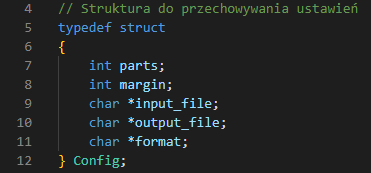
\includegraphics[width=0.65\linewidth, center]{img/config.png}
    
        \item \texttt{Input} \\
        Przechowywanie informacji pobranych z pliku wejściowego. Informacje te są później wykorzystywane do utworzenia macierzy sąsiedztwa oraz wypisywania danych do pliku wyjściowego.
    
        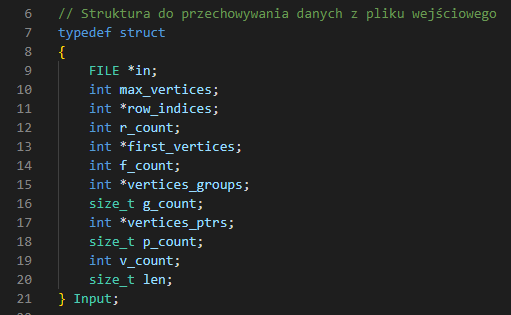
\includegraphics[width=0.75\linewidth, center]{img/input.png}

        \item \texttt{LanczosEigenV} \\
        Przechowywanie zmiennych do metody Lanczosa oraz do obliczania wartości własnych, przybliżonych wektorów własnych macierzy Laplace'a grafu oraz do podziału grafu.
    
        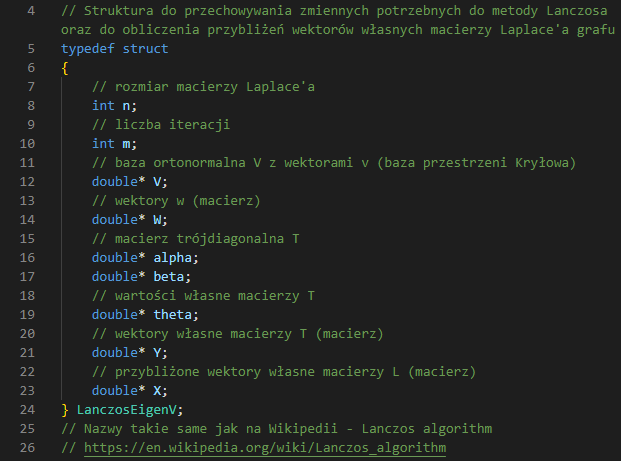
\includegraphics[width=0.825\linewidth, center]{img/lanczoseigenv.png}

        \item \texttt{Result} \\
        Przechowywanie zmiennych do wypisania wyniku w pierwszej linijce pliku wyjściowego.
    
        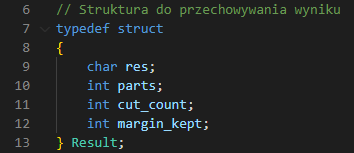
\includegraphics[width=0.825\linewidth, center]{img/result.png}
    
    \end{itemize}

    
    
    \subsection{Najważniejsze funkcje}
    
    \begin{itemize}
    
        \item \texttt{parse\_args} \\
        Obsługa argumentów. Zapisanie konfiguracji do obiektu struktury Config. Sprawdzenie i poprawa rozszerzenia pliku wyjściowego dla ustawionego formatu. \\\\      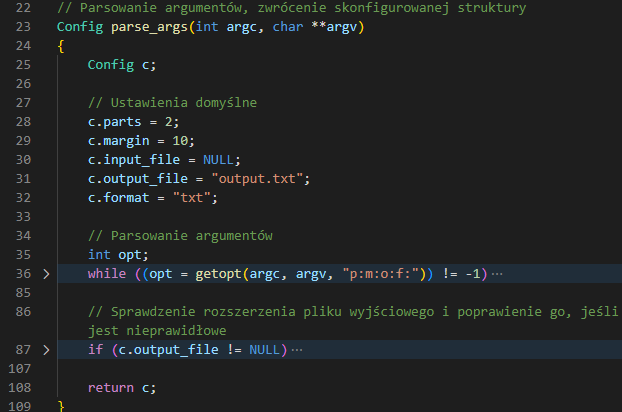
\includegraphics[width=0.8\linewidth, center]{img/parse_args.png}

        \item \texttt{read\_input} \\
        Wczytanie danych z pliku wejściowego do obiektu struktury Input. \\\\      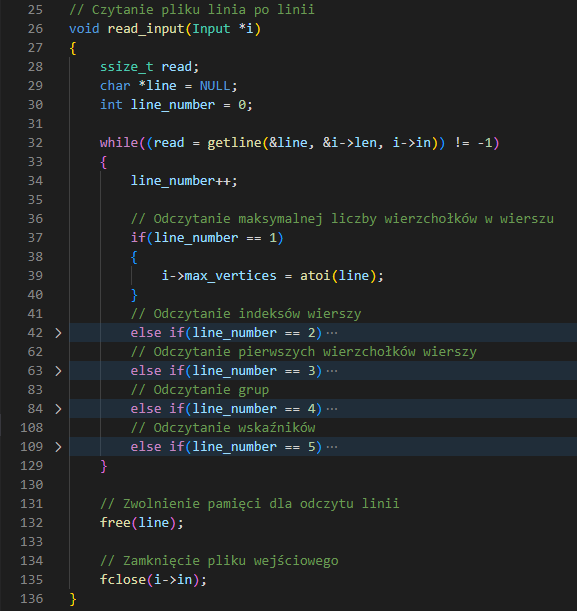
\includegraphics[width=0.8\linewidth, center]{img/read_input.png}
        
        \item \texttt{get\_adjacency\_matrix} \\
        Zapisanie grafu w formie macierzy sąsiedzywa. \\\\      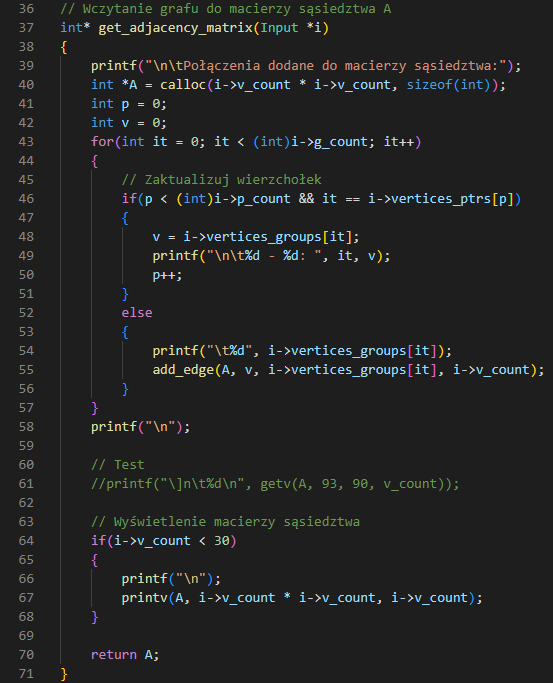
\includegraphics[width=0.8\linewidth, center]{img/get_adjacency_matrix.png}
        
        \item \texttt{calc\_laplacian} \\
        Obliczenie macierzy Laplace'a grafu. \\\\
        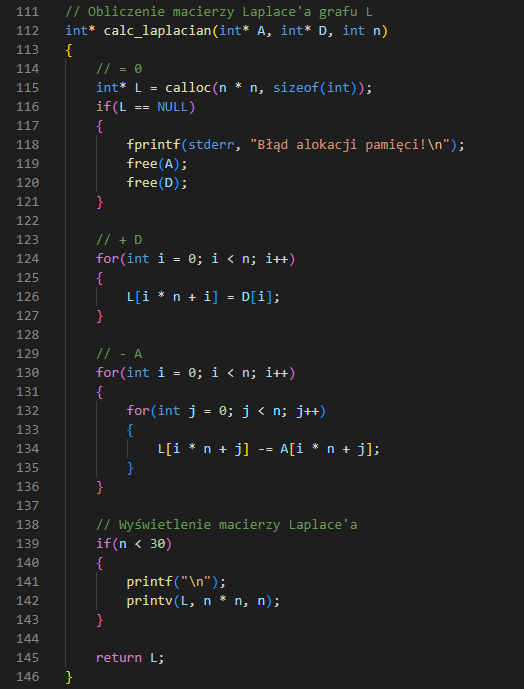
\includegraphics[width=0.8\linewidth, center]{img/calc_laplacian.png}
        
        \item \texttt{lanczos} \\
        Algorytm Lanczosa - przekształcenie problemu obliczenia wartości wektorów własnych macierzy Laplace'a na ich obliczenie dla macierzy trójdiagonalnej. \\\\
        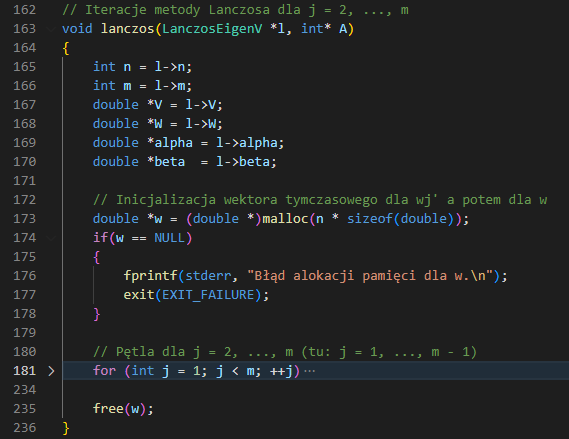
\includegraphics[width=0.8\linewidth, center]{img/lanczos.png}

        \item \texttt{qr\_algorithm} \\
        Obliczenie wartości wektorów własnych dla macierzy trójdiagonalnej. \\\\
        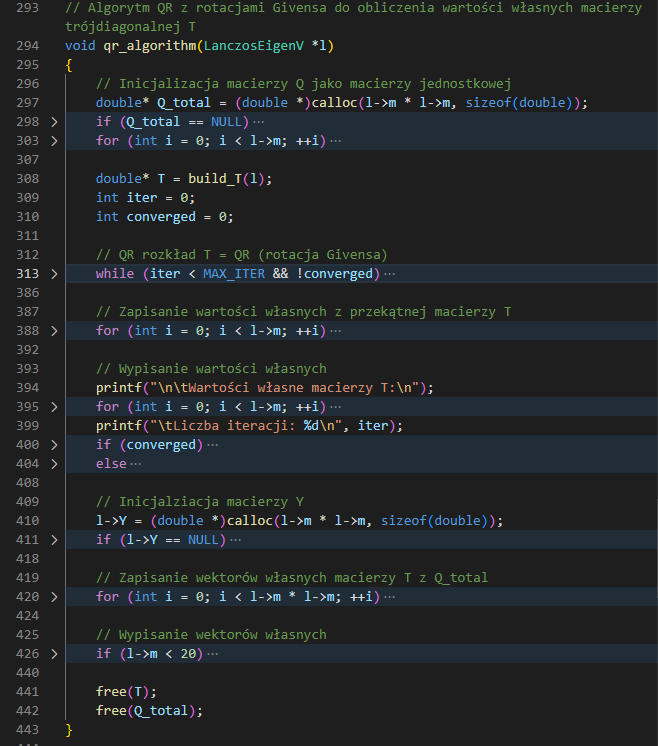
\includegraphics[width=0.8\linewidth, center]{img/qr_algorithm.png}
        
        \item \texttt{clusterization} \\
        Algorytm klasteryzacji - podziału wierzchołków na grupy w oparciu o wartości wektorów własnych macierzy Laplace'a grafu. \\\\
        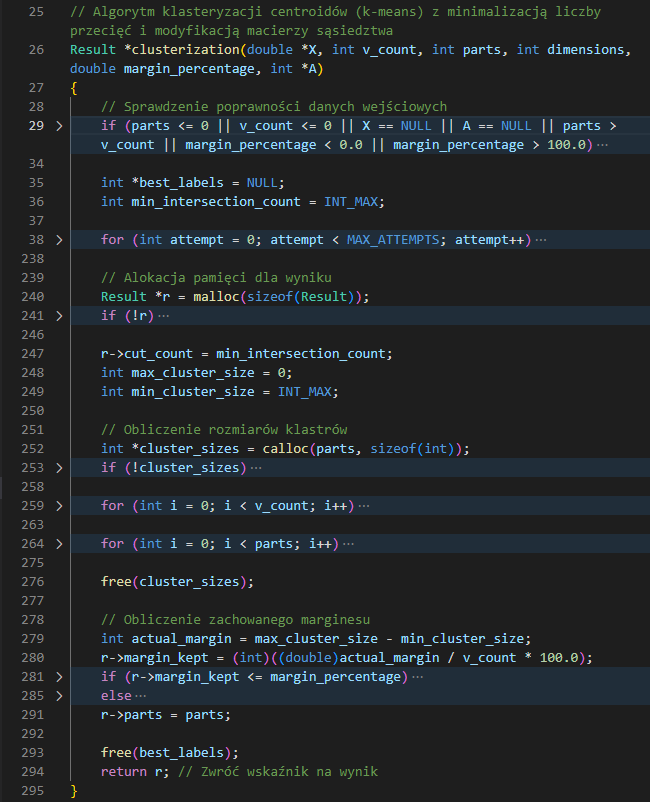
\includegraphics[width=0.8\linewidth, center]{img/clusterization.png}
        
        \item \texttt{write\_output} \\
        Wypisanie pliku wyjściowego z wynikiem i podzielonym grafem w odpowiednim formacie. \\\\
        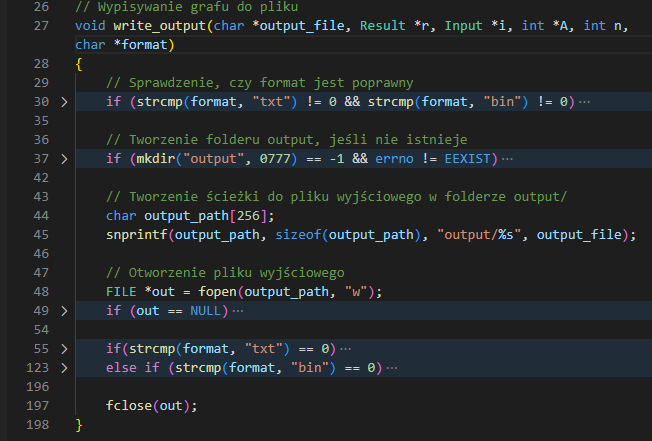
\includegraphics[width=0.8\linewidth, center]{img/write_output.png}
        
    \end{itemize}
    
    
    
    \subsection{Pliki wejściowe i wyjściowe}

        \subsubsection{Plik wejściowy (\texttt{.csrrg})}

        Program akceptuje pliki wejściowe z rozszerzeniem \texttt{.csrrg}. Format pliku składa się z pięciu sekcji, zapisanych w kolejnych linijkach:
        \begin{enumerate}
            \item Maksymalna liczba wierzchołków w dowolnym wierszu macierzy (graf może mieć wiersze o mniejszej liczbie sąsiadów, ale nie większej).
            \item Lista sąsiadów wszystkich wierzchołków, zapisana sekwencyjnie.
            \item Wskaźniki (indeksy) na początki list sąsiedztwa dla poszczególnych wierzchołków.
            \item Lista grup wierzchołków połączonych krawędziami (reprezentacja krawędzi).
            \item Wskaźniki na początki grup węzłów z poprzedniej listy.
        \end{enumerate}
        \textbf{Przykład:}
        \begin{center}
            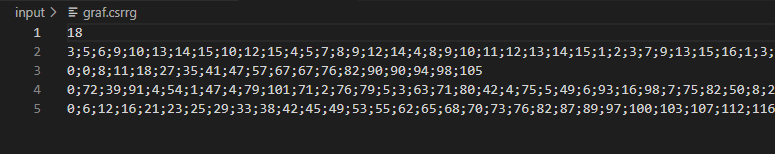
\includegraphics[width=1\linewidth]{img/grafcsrrg.png}
        \end{center}


        \subsubsection{Plik wyjściowy (\texttt{.txt} / \texttt{.bin})}
    
        Po przetworzeniu danych program zapisuje wynik do pliku wyjściowego w formacie tekstowym lub binarnym.
        \begin{itemize}
            \item \textbf{Pierwsza linijka} zawiera wynik działania programu w formacie: \\
            \texttt{<wynik (S - sukces, F - porażka)> <liczba\_części> <liczba\_przecięć> <zachowany\_margines>} \\
            Przykład: \texttt{S 3 2 5}
            \item \textbf{Kolejne linie} opisują strukturę grafu w tym samym formacie co plik wejściowy
            \item \textbf{Format binarny} (\texttt{.bin}) zapisuje te same informacje co plik tekstowy, lecz w postaci binarnej za pomocą funkcji \texttt{fwrite}, co umożliwia szybsze wczytywanie i mniejszy rozmiar pliku. Przed wypisaniem każdej tablicy podawana jest liczba elementów do poprawnego odczytu.
        \end{itemize}
        Przykład fragmentu pliku tekstowego:
        \begin{center}
            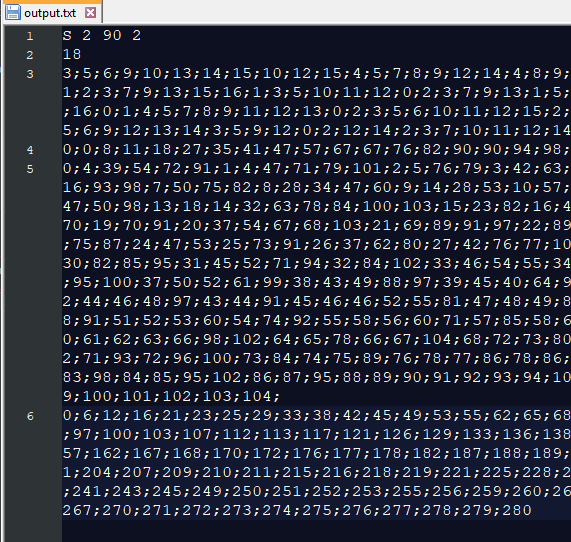
\includegraphics[width=0.8\linewidth]{img/outputtxt.png}
        \end{center}
        Przykład fragmentu pliku binarnego:
        \begin{center}
            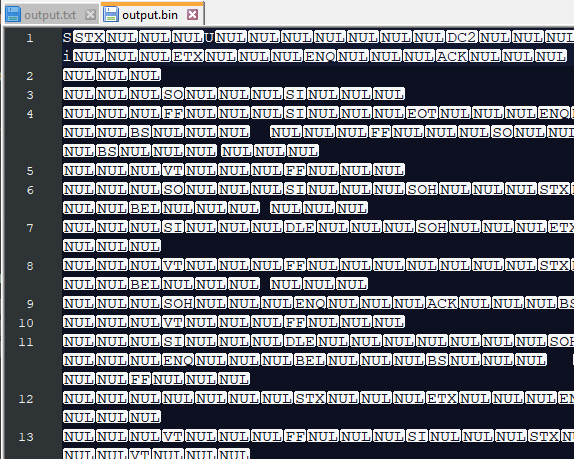
\includegraphics[width=0.8\linewidth]{img/outputbin.png}
        \end{center}



    \subsection{Testy}

    \subsubsection{Test 1: Funkcje \texttt{dot\_product}, \texttt{norm} i \texttt{mat\_vec\_multiply}}
    Pierwszy test sprawdza działanie funkcji do obliczania iloczynu skalarnego, normy wektora oraz mnożenia macierzy przez wektor. W ramach testu obliczono:
    \begin{itemize}
        \item Iloczyn skalarny wektorów \texttt{v1} i \texttt{v2}.
        \item Normę wektora \texttt{v1}.
        \item Wynik mnożenia macierzy \texttt{M} przez wektor \texttt{v1}.
    \end{itemize}
    
    \subsubsection{Test 2: Funkcje \texttt{orthogonalize} i \texttt{normalize}}
    
    Drugi test weryfikuje działanie funkcji odpowiedzialnych za ortogonalizację i normalizację wektorów. Sprawdzono:
    \begin{itemize}
        \item Ortogonalizację wektora \texttt{v} względem wektora \texttt{V1}.
        \item Normalizację wektora \texttt{v} oraz wektora \texttt{u}.
        \item Obsługę błędów dla próby normalizacji wektora zerowego.
    \end{itemize}
    
    \subsubsection{Test 3: Metoda Lanczosa, algorytm QR i dzielenie}
    
    Trzeci test dotyczy implementacji metody Lanczosa oraz algorytmu QR. Sprawdzono:
    \begin{itemize}
        \item Inicjalizację i normalizację wektora \texttt{v1}.
        \item Obliczenie wartości własnych i wektorów własnych macierzy Laplace'a grafu.
        \item Dzielenie grafu na dwie części.
    \end{itemize}
    Wszystkie testy zakończyły się pomyślnie.



    \section{Uruchomienie}

    Aby skompilować i uruchomić program, należy posiadać zainstalowane narzędzia:
    \begin{itemize} \item \texttt{gcc} – kompilator języka C, \item \texttt{make} – narzędzie do automatyzacji procesu kompilacji. \end{itemize}
    Proces kompilacji jest zautomatyzowany za pomocą pliku \texttt{Makefile}. Aby skompilować projekt, wystarczy w terminalu wydać polecenie 'make'.
    Po zakończeniu kompilacji, aby usunąć pliki wygenerowane podczas procesu (np. pliki obiektowe, pliki wykonywalne), można użyć polecenia 'make clear' lub 'make clear'.
    Polecenie \texttt{make clean} usunie pliki, które zostały utworzone w wyniku kompilacji, umożliwiając "czyste" ponowne zbudowanie projektu w przyszłości.
    Aby uruchomić program, należy postępować zgodnie z instrukcjami przedstawionymi w sekcji Flagi i argumenty. Przykład uruchomienia programu:
    \begin{center}
        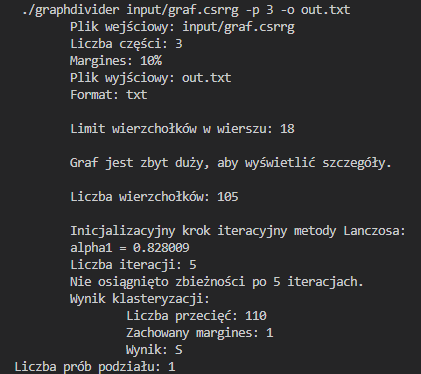
\includegraphics[width=0.5\linewidth]{img/uruchomienie.png}
    \end{center}
    W pliku wyjściowym zostaje zapisany rezultat oraz informacje o podzielonym grafie:
    \begin{center}
        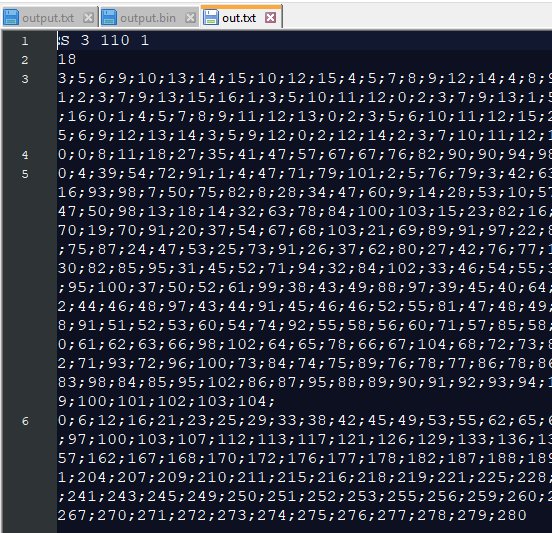
\includegraphics[width=0.75\linewidth]{img/uruchomienie2.png}
    \end{center}
    Przykład uruchomienia programu z wyjściem binarnym:
    \begin{center}
        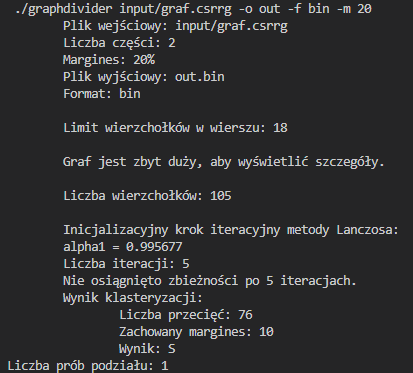
\includegraphics[width=0.5\linewidth]{img/uruchomienie3.png}
    \end{center}
    \begin{center}
        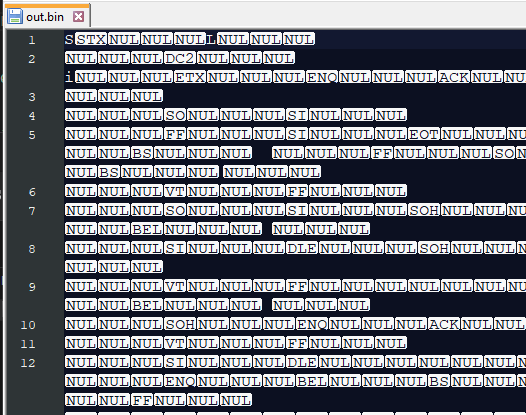
\includegraphics[width=0.75\linewidth]{img/uruchomienie4.png}
    \end{center}



    \section{Problemy i możliwe usprawnienia}
    Podczas pracy nad programem napotkano kilka istotnych problemów:
    \begin{enumerate}
        \item \textbf{Nieoptymalna liczba przecięć:} Liczba przecięć nie zawsze jest optymalna. Niedokładne przybliżenia wartości własnych mogą prowadzić w konsekwencji do nieoptymalnego podziału.
        \item \textbf{Problemy z większymi grafami:} Przy zastosowaniu metody Lanczosa do większych grafów mogą wystąpić problemy związane z wydajnością obliczeniową i stabilnością numeryczną. Dzielenie większych grafów trwa długo.
        \item \textbf{Optymalizacja przechowywania macierzy:} Przechowywanie macierzy w tablicach dynamicznych jest nieefektywne w przypadku macierzy rzadkich, w których przechowuje się mnóstwo zer. Zamiast tego, warto by było rozważyć zastosowanie jednego z popularnych formatów przechowywania macierzy rzadkich, przykładowo Compressed Sparse Row (CSR).
    \end{enumerate}
    
    


\begin{thebibliography}{9}

\bibitem{youtube_video}
Leonid Zhukov, \textit{Lecture 7. Graph partitioning algorithms.}, YouTube, 24 luty 2021, Dostępny na 1 kwietnia 2025 w: \url{https://youtu.be/zZae_C2BU_4}

\bibitem{laplacian_matrix}
\textit{Laplacian matrix}, Wikipedia, Dostępne na 1 kwietnia 2025 w: \url{https://en.wikipedia.org/wiki/Laplacian_matrix}

\bibitem{lanczos}
\textit{Lanczos algorithm}, Wikipedia, Dostępne na 1 kwietnia 2025 w:
\url{https://en.wikipedia.org/wiki/Lanczos_algorithm}

\bibitem{k-means}
\textit{Algorytm centroidów}, Wikipedia, Dostępne na 1 kwietnia 2025 w:
\url{https://pl.wikipedia.org/wiki/Algorytm_centroid%C3%B3w}

\end{thebibliography}



\end{document}
